\section{Introduction and Overview (Arek)}

To realize the promise and prospects of a Big Data society and avoid its security and confidentiality perils, institutions are updating operational frameworks governing business, legal, and technical dimensions of their internal organization and interactions with the outside world.
The control points traditionally relied upon as part of corporate governance, management oversight, legal compliance, and enterprise architecture must evolve and expand to match operational frameworks for Big Data.
An operational framework used for a Big Data driven organization requires a balanced set of institutional controls.
These institutional controls must support and reflect greater user control over personal data and large scale interoperability for data sharing between and among institutions.
Core capabilities of these controls include responsive rule-based systems governance and fine-grained authorizations for distributed rights management.
In the following sections we explore the emergence of the Big Data Society, outline the ways to support it in the institutional context, and draft the future directions of research and development.

\section{The New Realities of Living in a Big Data Society (Arek)}

Sustaining a healthy, safe and efficient society is a scientific and engineering challenge that goes back to the 1800s, when the Industrial Revolution spurred rapid urban growth, creating huge social and environmental problems.
Then the remedy was to build centralized networks that delivered clean water and safe food, enabled commerce, removed waste, provided energy, facilitated transportation, and offered access to centralized healthcare, police, and educational services.
Those networks formed a backbone of the society as we know it today.

But these century-old solutions are becoming increasingly obsolete and inefficient.
We have cities jammed with traffic, world-wide outbreaks of disease that are seemingly unstoppable, and political institutions that are deadlocked, unable to act.
We face the challenges of global warming, uncertain energy, water, and food supplies, and a rising population that will require building one thousand new cities of a million people each in order just to stay even. \comment{AS}{citation?}

It does not have to be this way.
We can have cities that are protected from pandemics, energy efficient, have secure food and water supplies, and have much better government.
To reach these goals, however, we need to radically rethink our approach.
Rather than static fixed systems, separated by function --- water, food, waste, transport, education, energy, etc. --- we must consider them as dynamic, data driven networks.
Instead of focusing only on access and distribution, we need dynamic, networked, and self-regulating systems that are driven by the needs and preferences of the citizens.

To ensure a sustainable future society, we must use our new technologies to create a \emph{nervous system} maintaining the stability of government, energy, and public health systems around the globe.
And our digital feedback technologies are capable of creating a level of dynamic responsiveness that our larger, more complicated modern society requires.
We must reinvent societies’ systems within a control framework: sensing the situation, then combining these observations with models of demand and dynamic reaction, and finally using the resulting predictions to tune the system to match the demands.

The engine that drives this new nervous system is Big Data: the newly ubiquitous digital data, now available about all aspects of human life.
We can now analyze patterns of human experience and idea exchange within the \emph{digital breadcrumbs} that we all leave behind as we move through the world: call records, credit card transactions, GPS location fixes, among others.
By recording are choices, these data tell the story of our lives.
This is very different from what we decide to put on Facebook or Twitter; our postings there are what we choose to tell people, edited according to the standards of the day.
Who we actually are is even more accurately determined by where we spend our time and which things we buy, rather than just what we say we do.

The process of analyzing the patterns within these digital breadcrumbs is called reality mining~\cite{eagle2006reality,pentland2009reality}, and through it we can learn an enormous amount about who we are.
The Human Dynamics research group at MIT have found that we can use them to tell if we are likely to get diabetes, or whether we are the sort of person who will pay back loans.\comment{AS}{citation?}
By analyzing these patterns across many people, we are discovering that we can begin to explain many things --- crashes, revolutions, bubbles --- that previously appeared to be random acts of God~\cite{pan2012decoding}.
For this reason the magazine Technology Review named our development of reality mining as one of the ten technologies that will change the world\cite{greene2008reality}. 

\section{The New Deal on Data (Arek)}

The digital breadcrumbs we leave behind provide clues about who we are and what we want.
This makes these personal data immensely valuable, both for public good and for private companies.
As European Consumer Commissioner Meglena Kuneva said recently, ``Personal data is the new oil of the Internet and the new currency of the digital world''~\cite{kuneva2009}.
This new ability to see the details of every interaction, however, can be used for good or for ill.
Therefore, maintaining protection of personal privacy and freedom is critical to our future success as a society.

A successful data driven society must be able to guarantee that our data will not be abused; perhaps especially that government will not abuse the power conferred by access to such fine-grain data.
To achieve the positive possibilities of a data driven society, we require the \emph{New Deal on Data}, workable guarantees that the data needed for public goods are readily available while at the same time protecting the citizenry~\cite{pentland2009reality}.
We must develop much more powerful and sophisticated tools for privacy and reach a consensus that allows us to use personal data to both build a better society and to protect the rights of the citizens.

The key insight that motivates the creation of the New Deal on Data is simply that our data are worth more when shared, because these aggregated data inform improvements in systems such as public health, transportation, and government.
For instance, we have demonstrated that data about the way we behave and where we go can be used to minimize the spread of infectious disease~\cite{madan2010social, pentland2009using}.
Our research has reported how we were able to use these digital breadcrumbs to track the spread of influenza from person to person on an individual level.
And if we can see it, we can stop it.
Here the result of sharing our personal data is that we can build a world where the threat of infectious pandemics is greatly diminished.

Similarly, if we are worried about global warming, these shared, aggregated data now show us how patterns of mobility relate to productivity~\cite{pan2013urban}.
In turn, this provides us with the ability to design cities that are more productive and, at the same time, more energy efficient.
But in order to be able to obtain these results and make a greener world, we need to be able to see the people moving around; this depends on many people willing to contribute their data, even if only anonymously and in aggregate.

While concrete examples such as better health systems and more energy efficient transportation systems motivate the New Deal on Data, there is an even greater public good that can be achieved by efficient and safe data sharing.
To enable sharing of personal data and experiences, we need secure technology and regulation that allow individuals to safely and conveniently share personal information with each other, with corporations, and with government.
Consequently, the heart of the New Deal on Data must be to provide both regulatory standards and financial incentives that entice owners to share data, while at the same time serving the interests of both individuals and society at large.
We must promote greater idea flow among individuals, not just corporations or government departments.

Unfortunately, today most personal data are siloed off in private companies and therefore largely unavailable.
Private organizations collect the vast majority of the personal data in the form of location patterns, financial transactions, phone and Internet communications, etc.
These data must not remain the exclusive domain of private companies, because then they are less likely to contribute to the common good.
These private organizations must be thus the key players in the New Deal on Data framework for privacy and data control.
Likewise, these data should not become the exclusive domain of the government, as this will not serve the public interest of transparency; we should be suspicious of trusting the government with such power.
Ultimately, the entities who should be empowered to share and make decisions about their data, are people themselves; people who are users, participants, citizens.

\section{Personal Data: Emergence of a New Asset Class (Thomas)}

It has long been recognized that the first step to promoting liquidity in land and commodity markets is to guarantee ownership rights so that people can safely buy and sell.
Similarly, the first step toward creating greater idea and idea flow (`idea liquidity’) is to define ownership rights.
The only politically viable course is to give individual citizens rights over data that are about them and in fact, in the European Union these rights flow directly from the constitution.
We need to recognize personal data as a valuable asset of the individual that is given to companies and government in return for services.

The simplest approach to defining what it means to “own your own data” is to draw an analogy with the English common law ownership rights of possession, use, and disposal:

• You have the right to possess data about you. Regardless of what entity collects the data, the data belong to you, and you can access your data at any time. Data collectors thus play a role akin to a bank, managing the data on behalf of their “customers.”

• You have the right to full control over the use of your data. The terms of use must be opt-in and clearly explained in plain language. If you are not happy with the way a company uses your data, you can remove the data, just as you would close your account with a bank that is not providing satisfactory service.

• You have the right to dispose of or distribute your data. You have the option to have data about you destroyed or re¬deployed elsewhere.

Individual rights to personal data must be balanced with the need of corporations and governments to use certain data–-account activity, billing information, and so on–-to run their day-to-day operations.
This New Deal on Data therefore gives individuals the right to possess, control, and dispose of copies of these required operational data, along with copies of the incidental data collected about you such as location and similar context.

Note that these ownership rights are not exactly the same as literal ownership under modern law, but the practical effect is that disputes are resolved in a different, simpler manner than would be the case for (as an example) land ownership disputes.

In 2007, one author (Pentland) first proposed the New Deal on Data to the World Economic Forum. 
Since then, this idea has run through various discussions and eventually helped shape the 2012 Consumer Data Bill of Rights in the United States, along with a matching declaration on Personal Data Rights in the EU.
These new regulations hope to accomplish the combined trick of breaking data out of the current silos, thus enabling public goods, while at the same time giving individuals greater control over data about them.
But, of course this is still a work in progress and the battle for individual control of personal data rages onward.

\section{Enforcing the New Deal on Data (Dazza)}

How can we enforce this New Deal?
The threat of legal action alone is important, but insufficient, because if you cannot see abuses then you cannot prosecute them.
Moreover, who wants more lawsuits anyway?
Enforcement can be addressed in significant ways without prosecution of public statute or regulation at all.
In many fields, companies and governments rely upon multi-party frameworks of agreed rules governing common business, legal and technical practices to create effective self-organization and enforcement.
These approaches hold promise as a method for using institutional controls to form a reliable operational framework balancing the needs for big data, privacy and access.

One current best practice is a system of data sharing called trust networks.
Trust networks are a combination of networked computers and legal rules defining and governing expectations regarding data.
With respect to data belonging to individuals, these networks of technical and legal rules keeps track of user permissions for each piece of personal data, and a legal contract that specifies both what you can and cannot do with the data and what happens if there is a violation of the permissions.
For example, in such a system all personal data can have attached labels specifying what the data can, and cannot, be used for.
These labels are exactly matched by the network's system rules and terms in legal contracts between all the participants stating penalties for not obeying the permission labels.
These rules can, and often do, reference or require audits of relevant systems and data use, demonstrating how traditional internal controls can be leveraged as part of the transition to more novel trust models.

Complete tracking and regulation of every aspect of a trust network is not the goal or even desirable in order to achieve effective enforcement.
Rather, the rules for a trust network align enforcement with the highest priority issues and those upon which trust of participants is premised.
The relevant issues arise from the dynamics of data flows, underlying trust models and contextual scenarios within which the networked data and the relationships of parties in the trust network. 
When a trust network involves use of personal data, then the user permissions and corresponding limits on use are fundamental to the trust model.
In this context, the permissions, including the provenance of the data, should require appropriate levels of audit.
A well designed trust network, elegantly integrating computer and legal rules, allows automatic auditing of data use and allows individuals to change their permissions and withdraw data.

Having system rules applicable to the networks, applications and data as well as all the services providers other intermediaries, and the users themselves is the mechanism for establishing and operating a trust network.
System rules are sometimes called operating regulations in the credit card context, or known as trust frameworks in the identity federations context, or trading parter agreements in a supply value chain context.
There are many general examples of multiparty shared architectural and contractual rules that share the generic characteristic of creating binding obligations and enforceable expectations on all participants in scalable networks.
Another common characteristic of the system rules design pattern is that the participants in the network can be widely distributed across very heterogeneous business ownership boundaries, legal governance structures and technical security domains.
Yet, the parties need not agree to conform all or most aspects of their basic roles, relationships and activities in order to connect to to systems of a trust network.
Cross-domain trusted systems must, by their nature, focus mandatory and enforceable rules narrowly upon the critical items that must be commonly agreed in order for that network to achieve it's purpose.

For example, institutions participating in credit card and automated clearinghouse debit transactional networks are subject to profoundly different sets of regulations, business practices, economic conditions and social expectations.
The network rules focus upon the topmost agreed items affecting interoperability, reciprocity, risk and revenue allocation.
The knowledge that fundamental rules are subject to enforcement actions is one of the foundations of trust as well as a motivation to prevent or address violations before they trigger penalties. 
A clear example of this approach can be found with the Visa Operating Rules, covering a vast global real-time network of parties that agree to rules governing their roles in the system as merchants, banks, transaction processors, individual or business card holders and other key system roles.

A system like this has made the interbank money transfer system among the safest systems in the world and the daily backbone for exchanges of trillions of dollars, but until recently such systems were only for the `big guys’.
To give individuals a similarly safe method of managing personal data, the Human Dynamics research group here at MIT, in partnership with the Institute for Data Driven Design, co-founded by John Clippinger and one author (Pentland), have helped build openPDS (open Personal Data Store) [fn: See http://openPDS.media.mit.edu for project information and https://github.com/HumanDynamics/openPDS for the open source code].
The openPDS system is a consumer version of a personal cloud trust network and we are now testing it with a variety of industry and government partners.
Soon, sharing your personal data could become as safe and secure as transferring money between banks.

[FN: The Human Dynamics Lab has applied the system rules approach to development of integrated business, technical architecture and rules large scale institutional use of personal data stores, available as an example under MIT's creative commons license by MIT, at: github.com/HumanDynamics/SystemRules and the Institute for Data Driven Design has published a guiding vision of digital common law, describing how these concepts can form the basis of next generation legal systems, available at: idcubed.org/??]

The capacity to apply the appropriate methods of enforcement for a trust network depend upon a clear understanding and agreement among parties about the purpose of the trusted system and the respective roles or expectations of those connecting is as participants.
Therefor, an anchor is needed to a clear context of a big data operational framework and institutional controls appropriate for access and confidentiality or privacy.
The following section posits the trust model and signature traits of such a context, through the lens of the New Deal on Data.

\section{Essential Elements of the New Deal of Data (Brian)}

To realize the promise and prospects of Big Data, and to avoid the associated privacy perils, we need a balanced set of institutional controls.
Theses controls must support and reflect a greater user control over personal data, as well as large scale interoperability for data sharing between and among institutions.

The core capabilities of theses controls should include responsive rule-based systems governance and fine grained authorizations for distributed rights management.

Our lives are embedded within institutions.
We are citizens of countries and cities, receive services from telecom operators, and search for things to buy in online stores.
Almost any action we perform generates data, and those recordings of our lives are an important part of the Big Data promise.
The data are not curated by us, but are collected `as is' - and reflect our lives.

Today, all the data people generate in the context of institutions are stored in closed silos. 
Mobility traces, for example, are owned by the phone providers, while musical preferences are stored and used by music services.

For these data to be useful to society, the silos must be opened, and the data must be used far more often than they are today.
If access to data for the purpose of creating value--either for the user or the society--is very limited, it does not matter how big the data is.
The value of the data lies not just in the fact that they exist.
Rather, it is the knowledge, understanding, and wisdom we gain from them that makes the data valuable.
It is an even bigger challenge to open up the data from multiple silos.
Accessing the multi-faced data, which exist under multiple jurisdictions, about people may be prohibitively difficult.
Silos are hard to crack open.
Such data, not just Big but Deep, covering multiple facets of a person's life, may be invaluable for research.

Recently, we have shown how challenging, but also possible, it is to open such institutional Big Data.
In the Data For Development (D4D) Challenge~\footnote{http://www.d4d.orange.com/home}, the telecom operator Orange opened access to a large dataset of call detail records (CDRs) from the Ivory Coast.
Working with the data as part of a challenge, teams of researchers came up with life-changing insights for the country.
The privacy of the people was protected not only by the technical means, such as removal of the Personally Identifiable Information (PIIs), but also by legal means, with the researchers signing an agreement they will not use the data for evil.
As we have seen in several cases, such as the Netflix Prize privacy disaster~\cite{narayanan2008robust} and other similar privacy breaches~\cite{sweeney2000simple}, true anonymization is extremely hard.
Some of the weight of privacy protection must rest on the legal framework.

Opening data from the silos by publishing static datasets is important, but it is only the first step.
We can do even more important things when the data is available in real time and can become part of a nervous system of a society.
Epidemics and traffic congestions can be monitored and prevented in real time, underpferoming students can be helped, and people with health risks can be treated before they get sick. The same data can be used for stalking, burglarizing one's home, and as a reason to charge people more for an insurance policy.

In the Unique in the Crowd project~\cite{de2013unique}, we have shown that even though human beings are highly predictable~\cite{song2010limits}, we are also very unique.
Having access to one dataset, it is easy to uniquely fingerprint someone based on just few datapoints, and use this fingerprint to discover their true identity.
The higher the resolution of the data, the better the data, the easier it gets.

The question of privacy in this context effectively becomes a question of control:

Who can release the data of one's movements?
To whom?
How much and how often?
The data are collected by the institution.
The data are about people and do not belong to them, they may not even be aware that they exist.
People cannot decide upon them, cannot review them.
People cannot delete them.
Very few parties can use the data, even if people wanted them to.
For systems to be truly data driven and capable of transitioning to the networked and highly dynamic assumptions of a big data economy, the key agreements reflected in trust networks must reflect a new deal.
The operating frameworks successful institutions are capable of balancing interests in access, confidentiality and every day reliance upon big data including personal and other sensitive information.
The institutional controls relevant to achieve, maintain and appropriately adapt these balances support and reflect adherence to the fair information practices.

[Footnote: HEW Report, OECD rendition, EU Directive, DHS/NSTIC version, MGL FIPA and culminating in New Deal on Data adaptation].

Within the existing legal frameworks, it is possible to change the vantage point of the data ownership and put the user, the entity about whom the data are, in control.
It may be a copy of the data living in the great silo, which is being given to the user.
The user would become the owner of their copy of the data, or whenever possible the original, in the old Common Law sense with the right to use, transfer, and delete the data.
An example of such a mechanism in an institutional context is Blue Button initiative~\footnote{http://www.healthit.gov/bluebutton}, where the patients can get a copy of their health records. 
Once the copy is with the user, they can do with it as they wish: give it to someone, make it public, do research on it, destroy it.

The users can accumulate data about themselves from multiple sources.
Information on healthcare records, mobility patterns, favorite movies, etc., all belong to the user and can be accessed based on their authorization.
This changes how and what data that can be obtained for the purpose of research and providing services.
Rather than gaining access to the movements of millions of people from a telcom operator, one can potentially gain access to a smaller number but of much richer datasets describing the users from the mobility, health, shopping perspectives.
New startups do not have to build the user profile from scratch, but can jump in offering competitive services based on the user's collected data.
Users can immediately get better services, using their data in new places.

The first, operational challenge of moving towards the end-user data ownership on a large scale, is to create an ecosystem where such user-owned data are noticed and accessed.
We are currently embedded in a feudal framework: Facebook owns the data generated by and about their users, and provides the access to them to the 3rd parties that user might or might have not authorized.
It is reasonably easy for users to download all their data from Facebook.
It is reasonably easy to put it on Dropbox or even create myself-API, becoming a self-hosted API to one's own personal data.
The challenge is to have clients to talk to this API and provide services, rather than going to Facebook for one's data.
Today, virtually no-one is ready to access user data directly from the user.
We have done a slightly better on the Internet scale with identity: one can deploy own OpenID server fairly easily, and many services will allow the user to sign in.
We should be heading in the same direction with data.

\section{Transitioning End-User Assent Practices (Arek)}

The way the user grants authorizations to the data she owns is not a trivial matter.
The flow of personal information, such as location data, purchases, health records, etc. can be very complex.
Every tweet, every geo-tagged picture, every phone call, and every purchase with credit card, provide the user's location not only to the primary service, but also to all the applications and services that have been authorized to access and re-use these data.
Implementation of such flows was a crucial part of the Web 2.0 revolution, realized with RESTful APIs, mashups, and authorization-based access.
The way the data travel between the services has however became arguably too complex for a user to handle and manage.

Increasing the amount of data the user controls and granularity of this control is meaningless if it cannot be exercised in an informed way.
For many years the End User License Agreements (EULAs), long incomprehensible texts, have been accepted blindly by the end user, who trust they have not agreed to anything harmful to them.
The process of granting the authorizations cannot be too complex, as it would prevent the user from understanding her decisions.
At the same time, it cannot be too simplistic, as it may not sufficiently convey the weight of the privacy-related decisions.
It is a challenge in itself, to build the end-user assent systems that allow the user to understand and adjust their privacy settings.
Complex EULAs do not promote the privacy of the users, effectively pushing them to pressing \emph{I Agree} in every presented window.
The consequences of those actions are not emphasized; as the data being collected is becoming increasingly complex and our computations more sophisticated, every act of sharing can lead to great benefits to the society, but also make the users vulnerable.

This gap between the interface, the single click, and the effect, can render the data ownership meaningless, if that click wrenches people and their data into systems and rules that are antithetical to fair information practices, such as is prevalent with todays end user licenses in cloud services or applications.
Managing the potentially long term and opposite dynamics fueled by old deal systems operating simultaneously with the new deal systems is an important design and migration challenge during the transition to a Big Data economy.
During this transition and after the New Deal on Data is no longer new, personal data must continue to flow in order to be useful.
Protecting the data of people outside of the user-controlled domain is very hard without a combination of cost effective and useful business practices, legal rules, and technical solutions.
For these reasons, the Human Dynamics group has focused upon and collaborated with partners to support the clarification of business, legal, and technical short- and longer-term viable solutions.

We envision Living Informed Consent, where the user is entitled to know what data is being collected about her by which entities, empowered to understand the implications of data sharing, and finally put in charge of the sharing authorizations.
We suggest the readers ask themselves a question: \emph{Which services know which city I am in today?}.
Google? Apple? Twitter? Facebook? Flickr?
This small application we have authorized a few years ago to access our Facebook check-ins and forgot since then? 
This is an example of a fundamental question related to use privacy and assent, and yet finding the answer to it may be surprisingly difficult.
We can hope that most of the services treat the data responsibly and according to user authorizations.
In the complex network of data flows however, services careless with the data or simply malicious, have a good chance of collecting users data.

It is clear that the promise of the Big Data can only be realized when the data is shared, available even more than it is today.
For this, the user herself should be put in the driver's seat and made decisions about who is authorized to see what and for what purpose.
To realize this, the solutions for making the user decisions well though-through must be designed and implemented.



\section{Business, Legal and Technical Dimensions of Big Data Systems (Dazza)}

When it comes to data intended to be accessible over networks–-whether big, personal or otherwise–-the traditional container of an institution makes less and less sense.
Institutional controls apply, by definition by or to some type of institutional entity such as a business, governmental or religious organization.
A combined view of the business, legal and technical facts and circumstances surrounding big data is necessary to know what access, confidentiality and other expectations exist.
The relevant contextual aspects of big data of one institutional is often profoundly different from that of another.
As more and more organizations use and rely upon big data, a single formula for institutional controls will not work for increasingly heterogeneous business, legal and technical environments in play.

Looking at an institution as a business, legal and technical “system” is one effective approach for dealing with the inherent complexity of managing heterogeneous and distributed networks of actors and interactions.
The business models, interface-point operational practices and relevant assumptions must be consistent and frequently carefully agreed at an executive level by and with institutions as part of the value exchange involving data and access to high value, mission critical or sensitive systems and services.
The applicable legal frameworks, common assumptions regarding likely allocation of liability and resolution of disputes in the event of losses and expected types of contracting practices need to reflect and support the business goals and purposes for the system and data.
When technical standards are selected, configured and applied to systems they too must support and reflect the business and legal dimensions and be supported and reflected by those dimensions.

Once a systems view is adopted, there is a tractable starting point to narrow or broaden the scope of view to see the smaller and larger systems and to make better and more effective use and control of big data.
Within a given institution, there may in fact be many different discernable institutions and corresponding systems and any given system of one institution will frequently in fact exist across many different discernable institutions. 
However, defining as a “system” the thing to which institutional controls apply provides an achievable and measurable basis for balancing privacy, access and other interests in big data.


\section{Digital Institutions: Redefining Institutional Controls (Thomas)}

{\small
{\bf These bullets summarize the flow of the text (to be deleted in the final edit):
\begin{itemize}
\item  A New vision of ``institutional controls''.
\item  Personal data as the driver for current digital economies and future digital institutions.
\item  The role of Computational Law.
\item  Defining Controls for Digital Institutions in terms of Trust Networks.
\item  The New Digital Institution Stack
\item  Digital Institutions that Self-Control: the Vision
\end{itemize}
(The text below is REV05 -- \today)
}
}
~~\\


The Internet offers a new opportunities for individuals,
communities and societies to interact based on 
self-organized governance.
Currently there is arguably an inequitable access to resources
on the Internet -- including to ``personal data'' -- 
where incumbent service providers
and digital technology providers seek to resist
open network dynamics and to maintain the old business models
which in the long term benefit only a fraction 
of the Internet population~\cite{greene2008reality,pentland2009reality,WEF2011}.
Current social networking platforms typically
rely upon proprietary business models that collect and sell
personal information about users,
inducing social distrust in these business models~\cite{HardjonoDeegan2014}.

The World Economic Forum has identified personal data
as a new asset class~\cite{WEF2011} upon which new forms of future
economic activities may develop.
In order for for data to attain its true potential in the future
global digital economy, new forms of {\em digital communities}
must be allowed to flourish and evolve over time.
Similar to communities that over time evolved into institutions that we know today 
(e.g. New York Stock \& Exchange Board from the early 1800's),
digital communities within the virtual space on the Internet
must be recognized as having a legitimate role in the global economy
and be permitted to evolve unhindered into 
future {\em digital institutions}~\cite{Clippinger2013-InternetDisruption}.

Self-governance of digital communities is an important
ingredient for these communities to develop into
digital institutions. 
In the work of~\cite{Clippinger2013-InternetDisruption}
the notion of self-governance means the use
of data access policies and data usage policies
that are implemented as {\em computational law},
where governance is built into the computational engines
that are part-and-parcel of the technologcal infrastructure
which implements the virtual community.


If personal data is to be considered as
a new assets class~\cite{WEF2011}
then there is a need for a new paradigm for considering
the role and importance of personal data in 
the world's digital institutions and digital economy of the future.
Correspondingly, for these emerging digital institutions
there needs to be a new paradigm for contemplating
the aspects of ``institutional control'' within these
future institutions.






\subsection{Personal Data Assets as the Foundation for Future Digital Institutions}

The promise of the economic benefits from equal access to 
data -- personal data, proprietary data, and government data --
is difficult to argue against.
Today an example of a revolutionary use of data
as the basis for new forms of economic activities
can be found in {\em virtual currencies} as exemplified
by systems such as {\em BitCoin}~\cite{BarberBoyen2012} and
{\em Ven}~\cite{Stalnaker2013}.
Like their brick-and-mortar equivalents,
these virtual currency systems can flourish
only if all the system participants have equal access
to data, be it market data, meta-data about the system itself,
provenance information regarding certain data,
or data that are used as assets to back certain currencies.
Just as inequitable access to market data today results
in an inefficient economic system,
the inequitable access to data on the Internet
-- including personal data that forms the basis for market data --
results in inefficient digital institutions.

The economic benefits derived from the availability of data
describing attributes of individuals (i.e. private information)
and data capturing the behavior of individuals is undeniable.
For example, the online consumer buying behavior now drives much
of the selling plans occurring at different seasons
of the annual retail market.
Similarly, one can argue that in the large social networks (e.g. Facebook)
the individual user is seen not a customer but rather as the product itself.
Thus, artificially divorcing the role
of an individual's data (as an asset form) from its economic role
(and therefore from its legal role) is short-sighted,
and subsequently denies the full potential of personal data
as an engine of the new global digital economy.


We also need a new paradigm for considering future digital institutions,
and aspects of their roles and responsibilities to their
stakeholders and to society at large.
This new paradigm must enable nascent digital institutions
(such as the virtual currency systems of today)
to consider the more subtle notions related to personal data
in the larger context of social interactions on the Internet.
Thus, in defining future ``institutional controls''
in the digital economy, digital institutions must embrace
the notions of the {\em provenance} of data,
of {\em ownership} of data (beyond copyright),
of {\em common-pool sharing} of  data within and across digital institutions,
of {\em self-governance} of digital institutions
and the use of artificial intelligence and machine learning
to effect computational law.

This new paradigm must accommodate the notion of personal data as 
common-pool resource~\cite{Ostrom2009} on an opt-in basis.
The foundational concept of the common-pool resource
was put forward by  Elinor Ostrom, the Nobel Laureate in
economics in 2009.
Ostrom identified key principles by which 
self-organized groups can manage common-pool resources in fair, 
sustainable ways.  
If data were to be regarded as a common-pool resource, 
Ostrom’s research shows how it would be possible 
for online groups to devise their own {\em data commons} 
to manage their personal data in their own interests.
This open the possibility for the data commons to be
the basis of self-organizing digital institutions,
where ``law'' would have a very different character from
the kinds law we know today.
The development of `` digital law'' or computational law
in self-organizing digital institutions
would enable users to devise new types
of legal contracts that are
computationally expressible and 
executable~\cite{HardjonoDeegan2014,Clippinger2013-InternetDisruption}.



\subsection{Trust Networks as the Legal Foundation of Digital Institutions}

A promising model for self-governing digital institutions based on computational law
is that of {\em Trust Networks}.
In simple terms, a trust network for digital communities represents
the community rules and operational regulations which all members
of the community are bound to from they time they opt-in into membership
of the community.

In the current brick-and-mortar economy there are a number of examples
of ``networks of trust'' that allow communities to pool resources and share risks.
In the international banking community the emergence
of the SWIFT network~\cite{SWIFTnetwork} 
(Society for Worldwide Interbank Financial Telecommunication) 
in the 1970s represented a major milestone for global banking.
The SWIFT network established a secure and reliable electronic network
that enables enables financial institutions worldwide 
to send and receive information about financial transactions.
Banks and financial institutions who wish to make use of the SWIFT network
must join the network by accepting a membership agreement.

Similarly, various identity federation consortium or organizations
have been established in the recent past with the aim of providing
a legal foundation to the creation, use and disposal of digital identities
on the Internet.
A recent example of such an organization is
the {\em Open Identity Exchange}~\cite{OIX-website}
whose aim is to create a {\em  Trust Framework} for identity federation
on the Internet
In digital identity systems, a trust framework
is a certification program that enables a party
who accepts a digital identity credential
(called the relying party) to trust the identity,
security, and privacy policies of the party
who issues the credential (called the identity
service provider) and vice versa~\cite{OIX-website}.

Currently efforts on legal ``trust frameworks''
are focused primarily on individual identity and identity federation.
However, we believe that a new legal foundation is
required for the personal data ecosystem and for
the various digital institutions that may utilize
personal data.
We believe a new view of the ``Internet stack''
needs to be introduced, where the stack
calls-out and recognizes the importance of personal data
and the crucial role of personal data stores or accounts.



\begin{figure*}[!t]
\centering
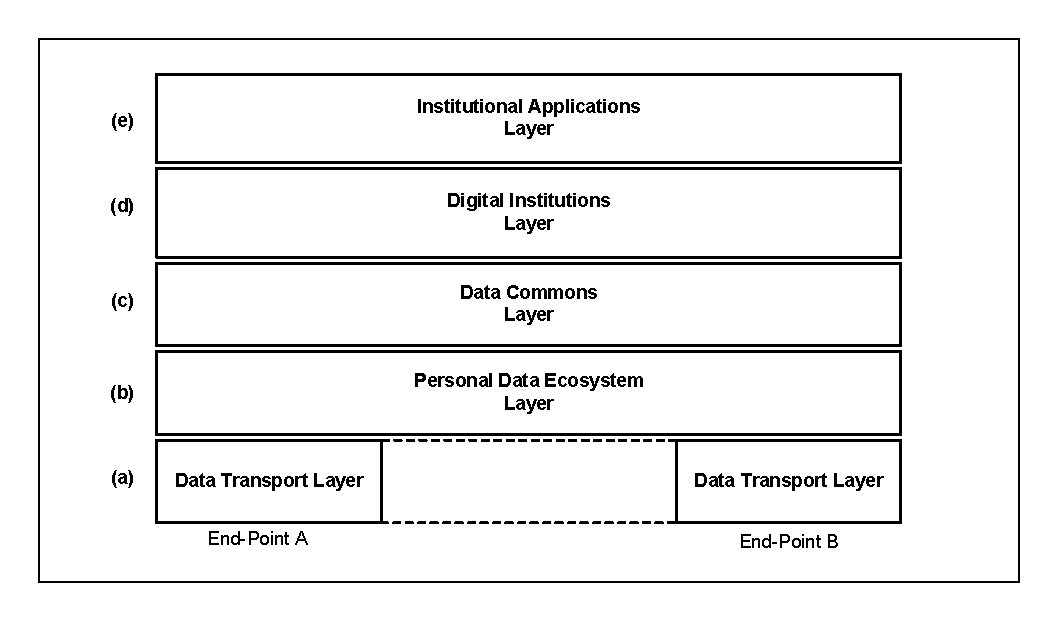
\includegraphics[width=7in]{figure-new-stack}
% where an .eps filename suffix will be assumed under latex, 
% and a .pdf suffix will be assumed for pdflatex; or what has been declared
% via \DeclareGraphicsExtensions.
\caption{A New Stack for Digital Institutions}
\label{fig:newstack}
\end{figure*}



\subsection{Digital Institutions: A New Stack for the Internet}

In order for society to obtain the benefits of 
personal data as a the new asset class,
a new personal data ecosystem must evolve where
every stakeholder has equitable access to data and other resources
within the ecosystem.
Such equitable access must be available not only to individuals
real-world communities,
but also to emerging digital communities and institutions.

We believe that a new vision is needed for seeing the 
Internet, personal data and digital institutions
in a consistent manner, something akin to the Internet
TCP/IP stack or the 7-layer ISO stack\footnote{
The network engineering view of the Internet sees
in in a 4-layer view, whereas the International standards
perceives the Internet consisting of 7 layers.
In reality these view converge on the core functions
of necessary for the Internet to function today.}.
We therefore propose that a new {\em digital institution stack} would
be useful for viewing the evolving personal data ecosystem.
Such a logical ``stack'' allows the stakeholders in the ecosystem
to understand better their roles in the ecosystem
and to define with more clarity the services or functions
that they offer, and the services
of other stakeholders upon which they rely.
Figure~\ref{fig:newstack} attempts to illustrate
one such new stack for the personal data ecosystem.

The proposed stack paves the way for legal trust frameworks
to be defined and developed for the personal data ecosystem,
for the ``pools of data'' as a common resource~\cite{Ostrom2009}
derived from personal data in the ecosystem,
and for the digital institutions that may evolve
from the communities that use these pools of data.
Finally, such a stack allows a  new {\em digital institutional controls}
to be defined for these emerging institutions.

The layers within this proposed new stack
are as follows (from bottom to top layers).
Note that the boundaries of the layers
are not strict in the sense that many
functions may in fact be implemented and operate across layers.
\begin{description}


\item[(a) Data Transport \& Infrastructure layer:]~\\
This layer is essentially the Internet of today
(e.g. Domain Name System, routing, autonomous systems, 
HTTP protocol, RESTful Web APIs, etc),
including all the ``big data'' related infrastructure
that exist today (e.g. virtualization, VM farms, etc)
or are being developed and brought to market
(e.g. homomorphic and functional encryption~\cite{BonehSahai2011},
differential privacy, etc).

We also include the current ``social network'' stack and
other semantic web~\cite{BernersLee1999} technologies.
The key aspect of this layer is that it is unaware of
(and hence agnostic to)
the semantics of personal data within PDS stores at the layer above,
and agnostic the relationships between entities to whom the data pertains.


\item[(b) Personal Data Ecosystem layer:]~\\
This layer pertains to the PDS end-points
within the personal data ecosystem,
the various services in the ecosystem and
the various transactions that occur among the end-points.
Today this layer is developing in an organic manner
and following the dictates of the market.

The following challenges should be logically
considered as part of this new layer:
\begin{itemize}
\item  Source and provenance of data-items or data-pools.
\item  Identity of stakeholders, and federation across stakeholders.
\item  De-personalization and de-identification of personal data.
\item  Relationships among data-items or data-pools.
\item  Log, audit and accountability systems that underlie the PDS stores.
\item  Protection and integrity of data and the PDS within which they reside.
\item  Computational policies and engines that regulate access
to data-pools.
\item  Others
\end{itemize}



\item[(c) Data Commons layer:]~\\
The data commons layer consists of all the ``pools of data''
-- built from personal data, proprietary data and government data --
that are accessible to digital institutions and
other organizations that accept the legal obligations
expressed in the trust framework governing a given pool of data.

Examples of pools of data may include data from the health sciences area~\cite{pentland2009using},
data from individuals that may have been donated
to certain {\em open data commons} initiatives,
historical data that are public (e.g. past stock market data),
and others.

The following are but a few of the challenges to be addressed
in this layer for pools of data:
\begin{itemize}
\item  A legal trust framework for a pool of data 9as a shared resource) developed
from trust frameworks covering individual data sources.

\item  A globally interconnected consent-management infrastructure
to allow individuals and organizations anywhere in the world
to contribute their data to a data pool as a common resource.

\item  Provenance and accountability infrastructures corresponding 
to the consent-management infrastructure.

\item  Others
\end{itemize}


Part of the trust framework may specifically
request the contributors to consent
to allowing the organization
to make this pool of data available to the public
through a standardized interface
under legal terms that are also defined in the
trust framework.
In other words, this pool of data
is now globally accessible to any entity
that accepts the legal terms of use specified
in the trust framework.



\item[(d) Digital Institutions layer:]~\\
When a set of entities seek to collaborate in the digital space
they may establish an online digital community,
which over time may evolve into 
a digital institution
which has obligations
to the members of the community and
to the owners (sources) of the data-pools that the community deploys.

The work of~\cite{HardjonoDeegan2014} 
on the {\em Open Mustard Seed} (OMS) project points to the potential
development of a globally interconnected virtual space
built atop of heterogeneous instances of virtual machines (VM)
operated by cloud providers and other virtualization service providers.
Thus, in effect an individual person can possess 
not only personal data stores
but also a digital space implemented by the set of VMs that he
or she legally owns.  These VMs are stitched together
to provide a unified view of the digital space
(or ``virtual room'') within which the individual
``lives'' and performs tasks.
Note that notion of a ``virtual room'' for individuals 
has been around for at least a decade now.
However, the OMS project
points to the possibility of a group of individuals
to jointly and remotely participating in a {\em common virtual space}
which runs one or more function-specific application.

One use-case of the OMS system pertains
to a group of local parents
who wish to establish a community-based car-pooling service
for their children living on the same street.
Each household is assumed to have an OMS instance,
which includes a personal data store (PDS)
that collects and stores personal data about the household,
including the location data (i.e. GPS data) from devices
belonging to members of the household.

In order to establish this community-based car-pooling service,
for example, a mother ``spins-up'' an OMS system instance
representing this community.
Each household participating in the service would then provide
consent-based access to the specific data items in their PDS store
within their OMS instance.
Using these sets of location data, these parents can now self-organize
a weekly schedule of shared car-pool service for their children,
with the confidence that their personal data is
shared only among the members of this community.

This same pattern of community-based social interaction
can be established for numerous purposes, and can be scaled-up
as needed.
Larger communities that are longer-term in their existence
may organically grow to resemble an institution 
where more complex rules and trust frameworks 
may be created to govern the institution.



\item[(e) Institutional Applications layer:]~\\
This layer may be subsumed by the layer below it,
but it is useful to logically consider it as a separate layer
because of the interesting cross-institutional use-cases
that may occur.

A good example of an ``application'' at this layer
that of the {\em virtual currency} proposition,
as exemplified by systems such as Ven~\cite{Stalnaker2013}
and BitCoin~\cite{BarberBoyen2012}.
A virtual currency exchange being backed and operated
by a group of brick-mortar institutions
may in fact be best described itself as a digital institution.

\begin{figure*}[!t]
\centering
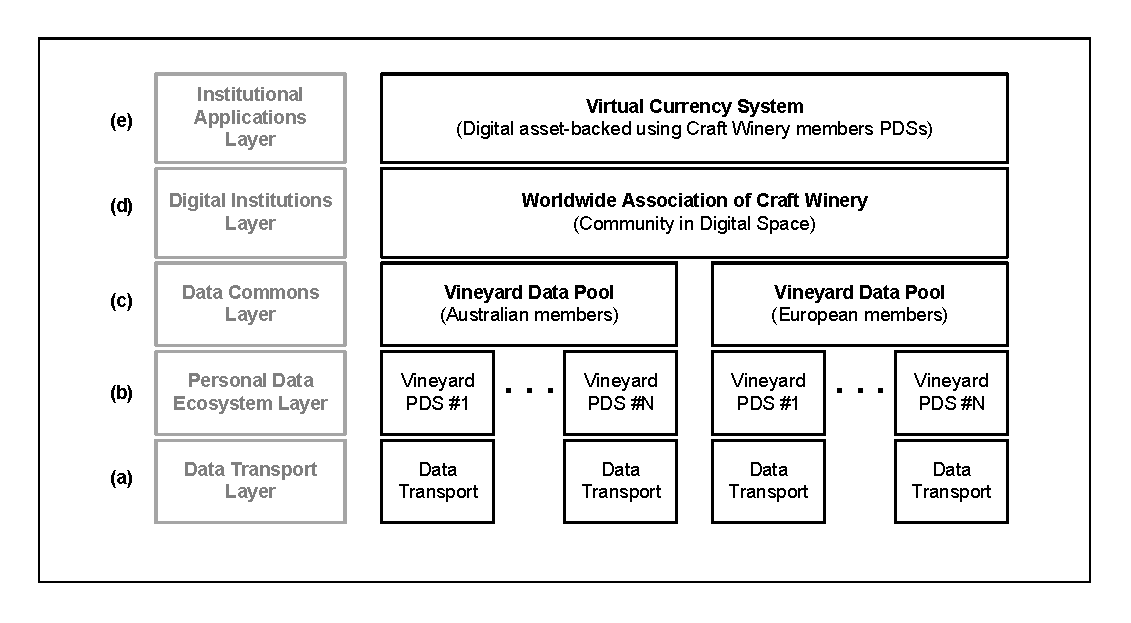
\includegraphics[width=7in]{figure-vineyard-stack}
% where an .eps filename suffix will be assumed under latex, 
% and a .pdf suffix will be assumed for pdflatex; or what has been declared
% via \DeclareGraphicsExtensions.
\caption{A New Stack for the Personal Data Ecosystem}
\label{fig:vineyard-stack}
\end{figure*}


Figure~\ref{fig:vineyard-stack} attempts to illustrate
the use-case of small craft vineyards around the world
that co-operate and trade among themselves in their
digital institution.  
Here, it is the wine-related trading that is
the institutional ``application'' in this layer.
This application may not be the sole application being
used by the craft winery community.
Another application could be a shared world-wide weather
database specific to the craft winery community.

The point here is that each digital institution
has the freedom to define and self-enforce their
legal trust framework by way of computational law technologies.
Furthermore, as shown in Figure~\ref{fig:vineyard-stack},
the participation of distinct data-pools (as independent
sets of data) allows each local digital community
to establish, manage and govern the usage of theor respective
data pools.
It also allows heterogeneous data -- and therefore more rich data --
to be shared within a global digital community.
Note that Figure~\ref{fig:vineyard-stack} also attempts to illustrate
the use of pools of data (created from personal data stores)
as the basis for creating an asset-backed virtual currency system.






\end{description}



\subsection{A new Paradigm for Digital Institutional Control}


~~\\
~~\\

















\section{Scenarios of Use in Context (Dazza)}

Supporting the effective development of institutional controls for big data requires an understanding of how to define and work with the applicable context surrounding the scenarios within which the big data exists. In particular, the New Deal on Data will require a set of Institutional Controls involving governance, business, legal and technical aspects that are knowable only with reference to the relevant context of a factually based scenario of use. The following scenarios demonstrate signature features of the New Deal on Data in various contexts and serve as an anchor to evaluate what Institutional Controls are well aligned.

\subsection{Example Scenario: Research Systems}

Computational Social Science (CSS) studies are based on data collected often with an extremely high resolution and scale. Using computational power combined with mathematical models, such data can be used to provide insights into human nature. Much of the data collected, for example mobility traces are sensitive and private; most individuals would feel uncomfortable sharing them publicly. The need for solutions to ensure the privacy of the individuals has grown alongside the data collection efforts.

The data collection in the CSS context is based on the informed consent of the participants. Countries have different bodies regulating such studies, for example Institutional Research Boards (IRBs) in the US. Although certain minimal requirements for implementing informed consent exist[TODO: reference], they are often not very well suited for the large-scale studies, where the amount and sensitivity of the data calls for sophisticated privacy controls. As the scale of the studies grows, in terms of the number of participants, collected bits per user, and duration, the EULA-style informed consent is no longer sufficient and makes it hard to claim that participants in fact expressed informed consent.

This year we have deployed a 1,000 phones study at Technical University of Denmark, where we handed out mobile phones to freshmen students in order to study their networks and social behavior in the important change moment of their lives, when they join the university. The study, called SensibleDTU, uses not only data collected from the mobile phones (location, Bluetooth-based proximity, call and sms logs etc.) but also data collected from social networks, questionnaires filled out by participants, behavior in economic games and so on. As the data is collected in the context of the university, there is potentially a big issues of students feeling obliged to participate in the study, feeling that their grades may depend on it, or that the data may influence their grades. In this context, we see the implementation of Living Informed Consent not only as a technical mean to put participants in control of the data we collect, but also to convey the message about the opt-in nature of the study, the boundaries of the data usage, and parties accessing the data.

It is not feasible to explain the terms and answer all the questions to all 1,000 students personally. The controls must be self-explanatory as much as possible, and guide the user from the first opening of the link to the study to the grant of the authorizations. At the same time, every click made by the user, should be an expression of an informed decision, so the user journey must be a balance of guidance and understanding. For this reason we have created a set of web applications, allowing the users to enroll into the study, express informed consent, and interact with their data.

As the study will last for several years, hopefully allowing us to see the life of a student from the very first friendships made until the graduation party, the consent must remain alive. It is again a matter of balance: we do not want the participants to feel under constant surveillance (as they are not, the data is used mostly in aggregated form), at the same time to remember that in fact, the data is being collected and used. We are still trying to understand how to achieve this equilibrium: how often should we remind the users about the collection effort? should they re-authorize applications from time to time? We see a great hope in the applications we create for the users to provide certain services, simple such as life-logging where they can see how active they are, what are their top places etc. and more advanced, such as artistic visualizations of their social networks. Making the user aware of the data by transforming them into value, can greatly benefit the privacy, making users constantly aware what is being collected, but also what kind of value they can get out of it.

When a study of such scale is deployed, the particular experiments and sub-studies may not be exactly defined from the very beginning. The initial deployment is a creation of a testbed, where shorter or longer experiments can take place; for example part of the population may participate in the experiment of quantifying the impact of feedback application on their activity levels. Being able to create such experiments in an efficient way is a huge value for the researchers. To do that in the most frictionless way, we give the users the choice to opt-in to those additional experiments, providing some financial or other benefits. This is only possible if there is a notion of identity of the participants, stronger and more useful than a piece of paper with a signature. This identity allows us to reach out to people, offer them additional experiments, and let them agree or disagree to them.

This touches upon the re-usability of data, as the new experiments may require additional data to be collected, but also have access to all the existing data, based on user authorization. We can imagine going even further, where entirely different studies can re-use participants data from a previous study based on their authorization. When the data are owned buy the users, they are free to authorize access to them to any party that requests it. We can see a New Deal on Data pattern here: rather than services (studies) talking to each other about the user data, they talk directly to the users, seeking their authorization. This can address a very important problem in the research context, the data re-use in a privacy-aware manner. Rather than publishing a static dataset, where the users have lost control over their data, live and fresh data can be continuously accessed by any study that the user agrees to be a part of.

Many studies will be willing to offer money or other value for the access to the data. Other will provide the user the opportunity to have new data collected. This way, the data collection becomes an opportunity for the user to enrich their personal dataset, and to benefit from it in the future. Join our study and we will provide you with a smartphone and collect your movement patterns for a year; we will do science and you will gain new data that can get you better value or deals in different services. You may now be eligible for a different study. Or your music recommendation may get better, because your music service can make a use of this extra data. Your data.

\subsection{Scenarios of Use Today, Tomorrow and the Day After}

By inquiring into and noting the four facets of relevant context described above, it is possible to describe the basic material contours of any scenario within which big data exists such that the operational framework and adequate approaches to access, use, confidentiality and other key interests can be sustainably balanced. In a commercial scenario the relevant people might be a consumer, merchants, banks, products manufacturers, third party app developers and individual members of that consumer’s bowling team. The relevant transactions might be a purchase of goods by the consumer from the merchant and the corresponding app that was embedded in the goods and the downstream transaction of involving the consumer now transacting with the merchant bowling alley and interacting with a bowling team, with whom activity and sports performance data are shared and aggregated and further mashed up. The rest of the context can be described for any given scenario and this all could be expressed specifically rather than by role simply by running a report from the system to indicate it was in fact John Doe, of openpds.org/owner/571 purchasing a smart bowling ball from Bowl-a-Tronic of bowlappgood.com/store/221 and so on for each party that played a role in the relevant scenario. The same techniques, used for scenarios in other economic sectors and social endeavors shed light on the fundamental nature and implications of big data and options for the use of operational frameworks acting across domains to balance privacy and access, among other intersts.

This book represents a high value opportunity to take stalk of the current state and dominant trends related to big data and help to illuminate important choices at a moment of early adoption, dynamic innovation and wide open possibilities. By contemplating the relevant contexts of todays scenarios of use in, say, the fields of education, entertainment, government, manufacturing, transportation and many other core anchors of human activity, we have traction to postulate how today’s prevailing trends are likely to result and what changes – perhaps quite small but of profound long term impact – could lead to materially different better outcomes. Consider that if the essence of the New Deal on Data were accepted today, or soon, the nature, tenor, capabilities and experience of living by future generations could be unrecognizably better. Simply extrapolate from the current anomalous practices regarding personal data and individual identity and push forward the timeline by 5, 10, 20 years and beyond. The current trajectory ends up with dystopian scenarios that effectively reverse hard fought but easily lost constitutional deal of the United States and social compact of common law and compatible societies.

By contrast, by adopting the New Deal on Data now it is entirely possible to enjoy a period of unprecedented prosperity and invention even before the new deal on data frameworks are formally launched. This is because the uncertainly and confusion about the basic premises and expectations around personal data and identity will be resolved and so investment and risk taking on a firm foundation can be unleashed. Many policy techniques can be used to make adoption of the new deal on data all but impossible to oppose on grounds of cost, disruption or over regulation. For instance, generous easy to implement support such as phase-in periods of many years, opportunities for delays and flexible approaches to adoption, etc.

\section{Future Research (Brian)}

Our traditional methods of testing and improving government, organizations, and so on are of limited use in building a data driven society. Even the scientific method as we normally use it no longer works, because there are so many potential connections that our standard statistical tools generate nonsense results.

The reason is that with such rich data, you can easily uncover misleading correlations. For instance, let’s imagine we discover that people who are unusually active are more likely to get the flu. This is a real example: when we examined the minute-by-minute behavior of a small university community – a real-time flow of gigabytes per day for an entire year – we noticed that an unusual level of running around often predicted onset of the flu. But if we can only analyze the data using traditional statistical methods, we have the problem of why is it true? Is it because flu virus makes us more active in order to spread itself more quickly? Or did interacting with many more people than usual make you more likely to catch the flu? Or is it something else? From the real-time stream of data by itself you just can’t know.

The point here is that normal analysis methods don't suffice to answer these sorts of questions, because we don’t know all the possible alternatives and so we can’t form a limited, testable number of clear hypotheses. Instead, we need to devise new ways to test the causality of connections in the real world. We can no longer rely on laboratory experiments; we need to actually do the experiments in the real world, and usually on massive, real-time streams of data.

\subsection{Research on Design and Deployment of Big Data Systems}

The highest value, lowest risks and overall best outcomes can be achieved most efficiently by applying top current research to design and deployment of the coming global wave of big data systems. To understand and address the unique problems and prospects affiliated with big data, the relevant context must be identified and corresponding rules-driven capabilities must be designed into the underlying systems.

People and/or rules engines can determine the right rules to apply to data when the right information is reliably attached to or logically associated with that data in a standard manner. Any system that can make, use, receive or share big data must be capable of associating provenance and purpose for all data in a common and actionable manner. Requiring a lot of narrative documentation and background about the nuances and circumstances surrounding every data set is both impractical and counterproductive. By contrast, a small amount metadata listing or reliably linking to the parties, transactions, systems and provenance of the data would suffice. This relevant context together

It is important for science and research to develop further solutions and options ensuring contextually appropriate rules can be applied by big data systems. For rules to be effectively applied, systems must not only be able to establish which rules apply but also support the right functional capabilities and have appropriate information structure, format and meta-data.

Today, computational social science can provide unprecedented insights into the business, legal and technical dimensions of big data driven systems. Harnessing these insights it will be possible to conduct research enabling common design patterns and reference implementations for responsive enterprise architectures that can orchestrate services and adapt rules based on dynamic real-time big data analytics. Advanced analytics reveals the reality of situations, and can be a powerful guide to the further optimization of financial management, user experience and control, conditions catalyzing innovation and other key inputs to overall economic impact.

Some capabilities will likely be essential to all big data systems, such as highly scalable active storage, standard methods for integration with other big data systems and a processing architecture enabling high speed statistical analytics. But there are and will continue to emerge multiple types of big data systems. Some functions or controls will likely be important - or even feasible - only for certain types of future systems. For instance, it is reasonable to expect some systems will specialize in enormous volumes of entirely non-personal data from many real-time sources (e.g. for soil science, materials engineering, astronomy, etc) while other big data systems will hinge upon mass quantities of highly sensitive personal information (e.g. for clinical medicine, education and life-long learning, social entertainment, etc).

While some capabilities, such as ingesting and processing astronomical data-sets, will be unique to only a subset of big data systems it is reasonable to anticipate that data will be increasingly cross-tabulated, merged and otherwise shared with other systems and data. It can be nearly impossible to conclusively predict for the entire life of a system what data will be received by, created in or transmitted from that system at the design phase. This prediction is all the harder to make when the systems are intended for big data.

The four contextual facets of people, interactions, technology and data were initially developed to provide a sound underpinning for the design of new big data and web 2.0 systems. The existing systems design and development processes of establishing business cases, use cases, agile stories, functional requirements, etc. do not reliably identify the factors most relevant to use of big data, especially in a web 2.0 massively distributed environment. The four facets can also be used to analyze appropriate, required or prohibited uses for existing big data systems. However, it can be difficult to extract the relevant information from or apply any effective control on systems used for big data but designed to achieve limited purposes in hierarchical closed environments.

Big data, by its nature, represents a new set of business, legal and technical capabilities and requirements. Most of the worlds systems today are not capable of ingesting, storing, using or dynamically flowing big data with other systems. Considering that a) big data is of high value immediately and higher value in the short and long terms, and b) the young but competitive marketplace of big data system components, platforms, applications and other solutions is a hotbed of innovation it can be predicted that a transition to big data systems will continue. The key observation is that virtually all big data systems have yet to be designed, implemented, customized or deployed. Institutions that are the current early adopters of today’s big data system will soon replace those systems and the rest of the world will adopt big data systems in phases over time. Based upon this observation,

\subsection{Research on Big Data for Design of Institutions}

Using massive, live data to design institutions and policies is outside of our normal way of managing things. We live in an era that builds on centuries of science and engineering, and the standard choices for improving systems, governments, organizations, and so on are fairly well understood. Therefore our scientific experiments normally need only consider a few clear alternatives (i.e., ‘plausible hypotheses’).

But with the coming of big data, we are going to be operating very much out of our old, familiar ballpark. These data are often indirect and noisy, and so interpretation of the data requires greater care than is usual. Even more importantly, a great deal of the data is about human behavior, and the questions are ones that seek to connect physical conditions to social outcomes. Until we have a solid, well-proven and quantitative theory of social physics, we won’t be able to formulate and test hypotheses in the way we can when we design bridges or develop new drugs.

Therefore, we must move beyond the closed, laboratory-based question-and-answering process that we currently use and begin to manage our society in a new way. We have to begin to test connections in the real world far earlier and more frequently than we have ever had to do before, using the methods my research group and I have developed for the Friends and Family study or the Social Evolution study. We need to construct Living Laboratories – communities willing to try a new way of doing things or, to put it bluntly, to be guinea pigs – in order to test and prove our ideas. This is new territory and so it is important for us to constantly try out new ideas in the real world in order to see what works and what doesn’t.

An example of such a Living Lab is the `open data city’ just launched by one author (Pentland) with the city of Trento in Italy, along with Telecom Italia, Telefonica, the research university Fondazione Bruno Kessler, the Institute for Data Driven Design, and local companies. Importantly, this Living Lab has the approval and informed consent of all its participants – they know that they are part of a gigantic experiment whose goal is to invent a better way of living. More detail on this Living Lab can be found at http://www.mobileterritoriallab.eu/

The goal of this Living Lab is to develop new ways of sharing data to promote greater civic engagement and exploration. One specific goal is to build upon and test trust-network software such as our openPDS (Personal Data Store) system . Tools such as openPDS make it safe for individuals to share personal data (e.g., health data, facts about your children) by controlling where your data go and what is done with them.

The specific research questions we are exploring depend upon a set of “personal data services” designed to enable users to collect, store, manage, disclose, share and use data about themselves. These data can be used for the personal self-empowerment of each member, or (when aggregated) for the improvement of the community through data commons that enable social network incentives. The ability to share data safely should enable better idea flow among individuals, companies, and government, and we want to see if these tools can in fact increase productivity and creative output at the scale of an entire city.

An example of an application enabled by the openPDS trust frame work is sharing of best practices among families with young children. How do other families spend their money? How much do they get out and socialize? Which preschools or doctors do people stay with for the longest time? Once the individual gives permission, our openPDS system allows such personal data to be collected, anonymized and shared with other young families safely and automatically.

The openPDS system lets the community of young families learn from each other without the work of entering data by hand or the risk of sharing through current social media. While the Trento experiment is still in its early days, the initial reaction from participating families is that these sorts of data sharing capabilities are valuable, and they feel safe sharing their data using the openPDS system.

The Trento Living Lab will let us investigate how to deal with the sensitivities of collecting and using deeply personal data in real-world situations. In particular, the Lab will be used as a pilot for the New Deal on Data and for new ways to give users control of the use of their personal data. For example, we will explore different techniques and methodologies to protect the users’ privacy while at the same time being able to use these personal data to generate a useful data commons. We will also explore different user interfaces for privacy settings, for configuring the data collected, for the data disclosed to applications and for those shared with other users, all in the context of a trust framework.
